\documentclass[12pt]{report}
\setlength{\textwidth}{6.5 in}
\setlength{\evensidemargin}{0 in}
\setlength{\oddsidemargin}{0 in}
\setlength{\textheight}{9.4 in }
\setlength{\topmargin}{-0.7 in}
\pagestyle{myheadings}
\markboth{\em EE264: Homework \#02}{\em EE264: Homework \#02}
\usepackage[pdftex]{graphicx} \usepackage{eso-pic}
\usepackage{amsmath}
\usepackage{amssymb}
\usepackage{graphicx}
\usepackage{ifthen}
\usepackage{tikz}
\usepackage{pgfplots}
\usepackage{array}  % for table column M
\usepackage{makecell} % to break line within a cell
\usepackage{verbatim}
\usepackage{epstopdf}
\usepackage{amsfonts}
\usepackage{xcolor}
\usepackage{subcaption}
\usepackage{pdfpages}
\usepackage{hyperref}
%\captionsetup{compatibility=false}
%\usepackage{dsfont}
\usepackage[absolute,overlay]{textpos}
\usetikzlibrary{calc, angles,quotes}
\usetikzlibrary{pgfplots.fillbetween, backgrounds}
\usetikzlibrary{positioning}
\usetikzlibrary{arrows}
\usetikzlibrary{pgfplots.groupplots}
\usetikzlibrary{arrows.meta}
\usetikzlibrary{plotmarks}
\usetikzlibrary{decorations.markings}

\DeclareGraphicsExtensions{.pdf,.eps,.png}

\DeclareMathOperator{\E}{\mathbb{E}} % expectation

\def\thickness{very thick}

\tikzset{
amark/.style 2 args={
	decoration={             
		markings, 
		mark=at position {0.5} with { 
			\arrow{stealth},
			\node[#2] {#1};
		}
	}, \thickness,
	postaction={decorate}
},
earlymark/.style 2 args={
	decoration={             
		markings, 
		mark=at position {0.25} with { 
			\arrow{stealth},
			\node[#2] {#1};
		}
	}, \thickness,
	postaction={decorate}
},
latemark/.style 2 args={
	decoration={             
		markings, 
		mark=at position {0.8} with { 
			\arrow{stealth},
			\node[#2] {#1};
		}
	}, \thickness,
	postaction={decorate}
},
zpath/.style={
	decoration={             
		markings, 
		mark=at position {0.5} with { 
			\arrow{stealth},
			\node[#1] {$z^{-1}$};
		}
	}, \thickness,
	postaction={decorate}
},
terminal/.style 2 args={draw,circle,inner sep=2pt,label={#1:#2}},
}


\newcommand\SimpleSys[4]{%
	\def\xin{#2}%
	\def\Hz{#3}%
	\def\yout{#4}
	\input{#1}%
}

\begin{document}
\thispagestyle{empty}
\begin{centering}
	{\large Stanford University}\\
	{\large EE 264: Digital Signal Processing}\\
	{\large Summer, 2018} \\
	\mbox{}\\
	{\large Homework \#02}\\
	\mbox{}\\
\end{centering}
\noindent Date assigned:  July 6, 2018 \hfill
Date due: July 13, 2018\\
\noindent \rule{6.5 in}{0.5pt}
%\mbox{}\\
\mbox{}\\ 
\noindent {\bf Reading:}  This assignment covers primarily the lecture on LTI systems, which correspond to chapters 5 and 6 of the textbook {\bf DTSP 3e}. \\

\noindent {\bf Homework submission:}  Please submit your solutions on Gradescope. Create a single .pdf file containing all your analytical derivations, sketches, plots, and Matlab code (if any). \\
\noindent
\rule{6.5 in}{0.5pt}
\mbox{}\\ 

\noindent {\bf Problem 1: (25 points)} 
A causal LTI system has the system function
\mbox{}\\ 

\begin{equation}
H(z) = \frac{(1-e^{j\pi/3} z^{-1})(1-e^{-j\pi/3}z^{-1})(1+(1/0.85)z^{-1})}{(1-0.9e^{j\pi/3} z^{-1})(1-0.9e^{-j\pi/3}z^{-1})(1+0.85z^{-1})}
\end{equation}
\mbox{}\\ 
\begin{description}
	\item{(a)} Plot the pole-zero diagram using Matlab's \texttt{zplane} function and indicate the region of convergence for the system function. 
	
	\textit{Hint:} Use the function \texttt{conv} to multiply out the denominator and numerator factors. The \texttt{conv} function is also used for the multiplication of polynomials.
	
	\item{(b)} Either plot or sketch the magnitude and phase responses of $H(e^{j\omega})$.
	
	\item{(c)} Either plot or sketch the group delay of $H(e^{j\omega})$. For the group delay you can use the Matlab function \texttt{grpdelay}. You may also numerically derivate the unwrapped phase to obtain the group delay.
	
	\item{(d)} State whether the following statements about $H(z)$ are true or false. Justify your answers. 
	\begin{enumerate}
		\item The system is stable
		\item The impulse response of that system approaches a non-zero value as $n\to\infty$.
		\item Since the system function has a pole at angle $\pi/3$ the magnitude of the frequency response has a peak at approximately $\omega=\pi/3$.
		\item The system is a minimum phase system.
		\item The system has a causal and stable inverse.
	\end{enumerate}
\end{description}
\mbox{}\\ 
\newpage

\noindent {\bf Problem 2: (25 points)} 

$H(z)$ is the system function for a \underline{stable} and \underline{causal} LTI system and is given by:
\begin{equation}
H(z) = \frac{(1-9z^{-2})(1+(1/3)z^{-1})}{(1-(1/3)z^{-1})}
\end{equation}

\begin{description}
	\item[(a)] $H(z)$ can be represented as a cascade of a minimum-phase system $H_{min}(z)$ and a unit-gain all-pass system $H_{ap}(z)$; i.e., $H(z) = H_{min}(z)H_{ap}(z)$. Determine a choice for $H_{min}(z)$ and $H_{ap}(z)$ and specify whether or not they are unique up to a scale factor.
	\item[(b)] Is the minimum-phase system, $H_{min}(z)$ in part (a) an FIR system? Explain.
	\item[(c)] For generalized linear phase FIR systems with \underline{real} coefficients, show that if $z = c$ is a zero, then $c^*, 1/c, 1/c^*$ must also be zeros. In words, zeros of generalized linear phase FIR systems appear in conjugate and conjugate reciprocal pairs.
	\item[(d)] Can $H(z)$ be represented as a cascade of a FIR generalized linear-phase system $H_{lin}(z)$ and an all-pass system $H_{ap2}(z)$; i.e., $H(z) = H_{lin}(z)H_{ap2}(z)$? If your answer is yes, determine $H_{lin}(z)$ and $H_{ap2}(z)$. If your answer is no, explain why such a representation does not exist.
\end{description}

\mbox{}\\ 
\noindent {\bf Problem 3: (25 points)} (adapted from several previous midterms)

Answer the following questions about the causal LTI systems having the pole-zero given in Figure~\ref{fig:pole-zero-diagram}.

In each case \underline{explain} why you chose the ones that you chose.

\begin{description}
	\item{(a) } Which systems are FIR systems? \\
	\hspace{10cm} (A)  \hspace{1cm}  (B)  \hspace{1cm}  (C) \hspace{1cm} (D) \hspace{1cm}  (E) \hspace{1cm} (F) \hspace{1cm} none \hspace{1cm}  all
	
	\item{(b) } Which systems are stable systems? \\
	\hspace{10cm} (A)  \hspace{1cm}  (B)  \hspace{1cm}  (C) \hspace{1cm} (D) \hspace{1cm}  (E) \hspace{1cm} (F) \hspace{1cm} none \hspace{1cm}  all
	
	\item{(c) } Which systems are \underline{probably}\footnotemark  all-pass systems, i.e., ${|H(e^{j\omega)}|}^2=$ constant for all $\omega$? \\
	\hspace{10cm} (A)  \hspace{1cm}  (B)  \hspace{1cm}  (C) \hspace{1cm} (D) \hspace{1cm}  (E) \hspace{1cm} (F) \hspace{1cm} none \hspace{1cm}  all
	
	\footnotetext{The word \underline{probably} is used because it is not possible to know the exact coordinates of the pole and zeros. However, you should make a favorable estimate of the locations when trying to match a property.}
	
	\item{(d) } Which systems are minimum-phase systems? \\
	\hspace{10cm} (A)  \hspace{1cm}  (B)  \hspace{1cm}  (C) \hspace{1cm} (D) \hspace{1cm}  (E) \hspace{1cm} (F) \hspace{1cm} none \hspace{1cm}  all
	
	\item{(e) } Which systems are \underline{probably} linear-phase systems? \\
	\hspace{10cm} (A)  \hspace{1cm}  (B)  \hspace{1cm}  (C) \hspace{1cm} (D) \hspace{1cm}  (E) \hspace{1cm} (F) \hspace{1cm} none \hspace{1cm}  all
	
	\item{(f) } Which systems have $H(e^{j\pi})=0$? \\
	\hspace{10cm} (A)  \hspace{1cm}  (B)  \hspace{1cm}  (C) \hspace{1cm} (D) \hspace{1cm}  (E) \hspace{1cm} (F) \hspace{1cm} none \hspace{1cm}  all
	
	\item{(g) } Which systems have \underline{lowpass} frequency response? \\
	\hspace{10cm} (A)  \hspace{1cm}  (B)  \hspace{1cm}  (C) \hspace{1cm} (D) \hspace{1cm}  (E) \hspace{1cm} (F) \hspace{1cm} none \hspace{1cm}  all
	
	\item{(h) } Which system has the shortest (least number of non-zero samples) impulse response? \\
	\hspace{10cm} (A)  \hspace{1cm}  (B)  \hspace{1cm}  (C) \hspace{1cm} (D) \hspace{1cm}  (E) \hspace{1cm} (F) \hspace{1cm} none \hspace{1cm}  all
	
	\item{(i) } Which systems have corresponding stable and causal inverse systems? \\
	\hspace{10cm} (A)  \hspace{1cm}  (B)  \hspace{1cm}  (C) \hspace{1cm} (D) \hspace{1cm}  (E) \hspace{1cm} (F) \hspace{1cm} none \hspace{1cm}  all
	
	\item{(j) } For the system labeled \textbf{C}, write the system function $H(z)$ as the product of a minimum phase function and an all-pass function. Assume that all the poles have radius 0.8, and the zeros outside the unit circle have radius 1.1.
\end{description}

\begin{figure}[h!]
	\centering
	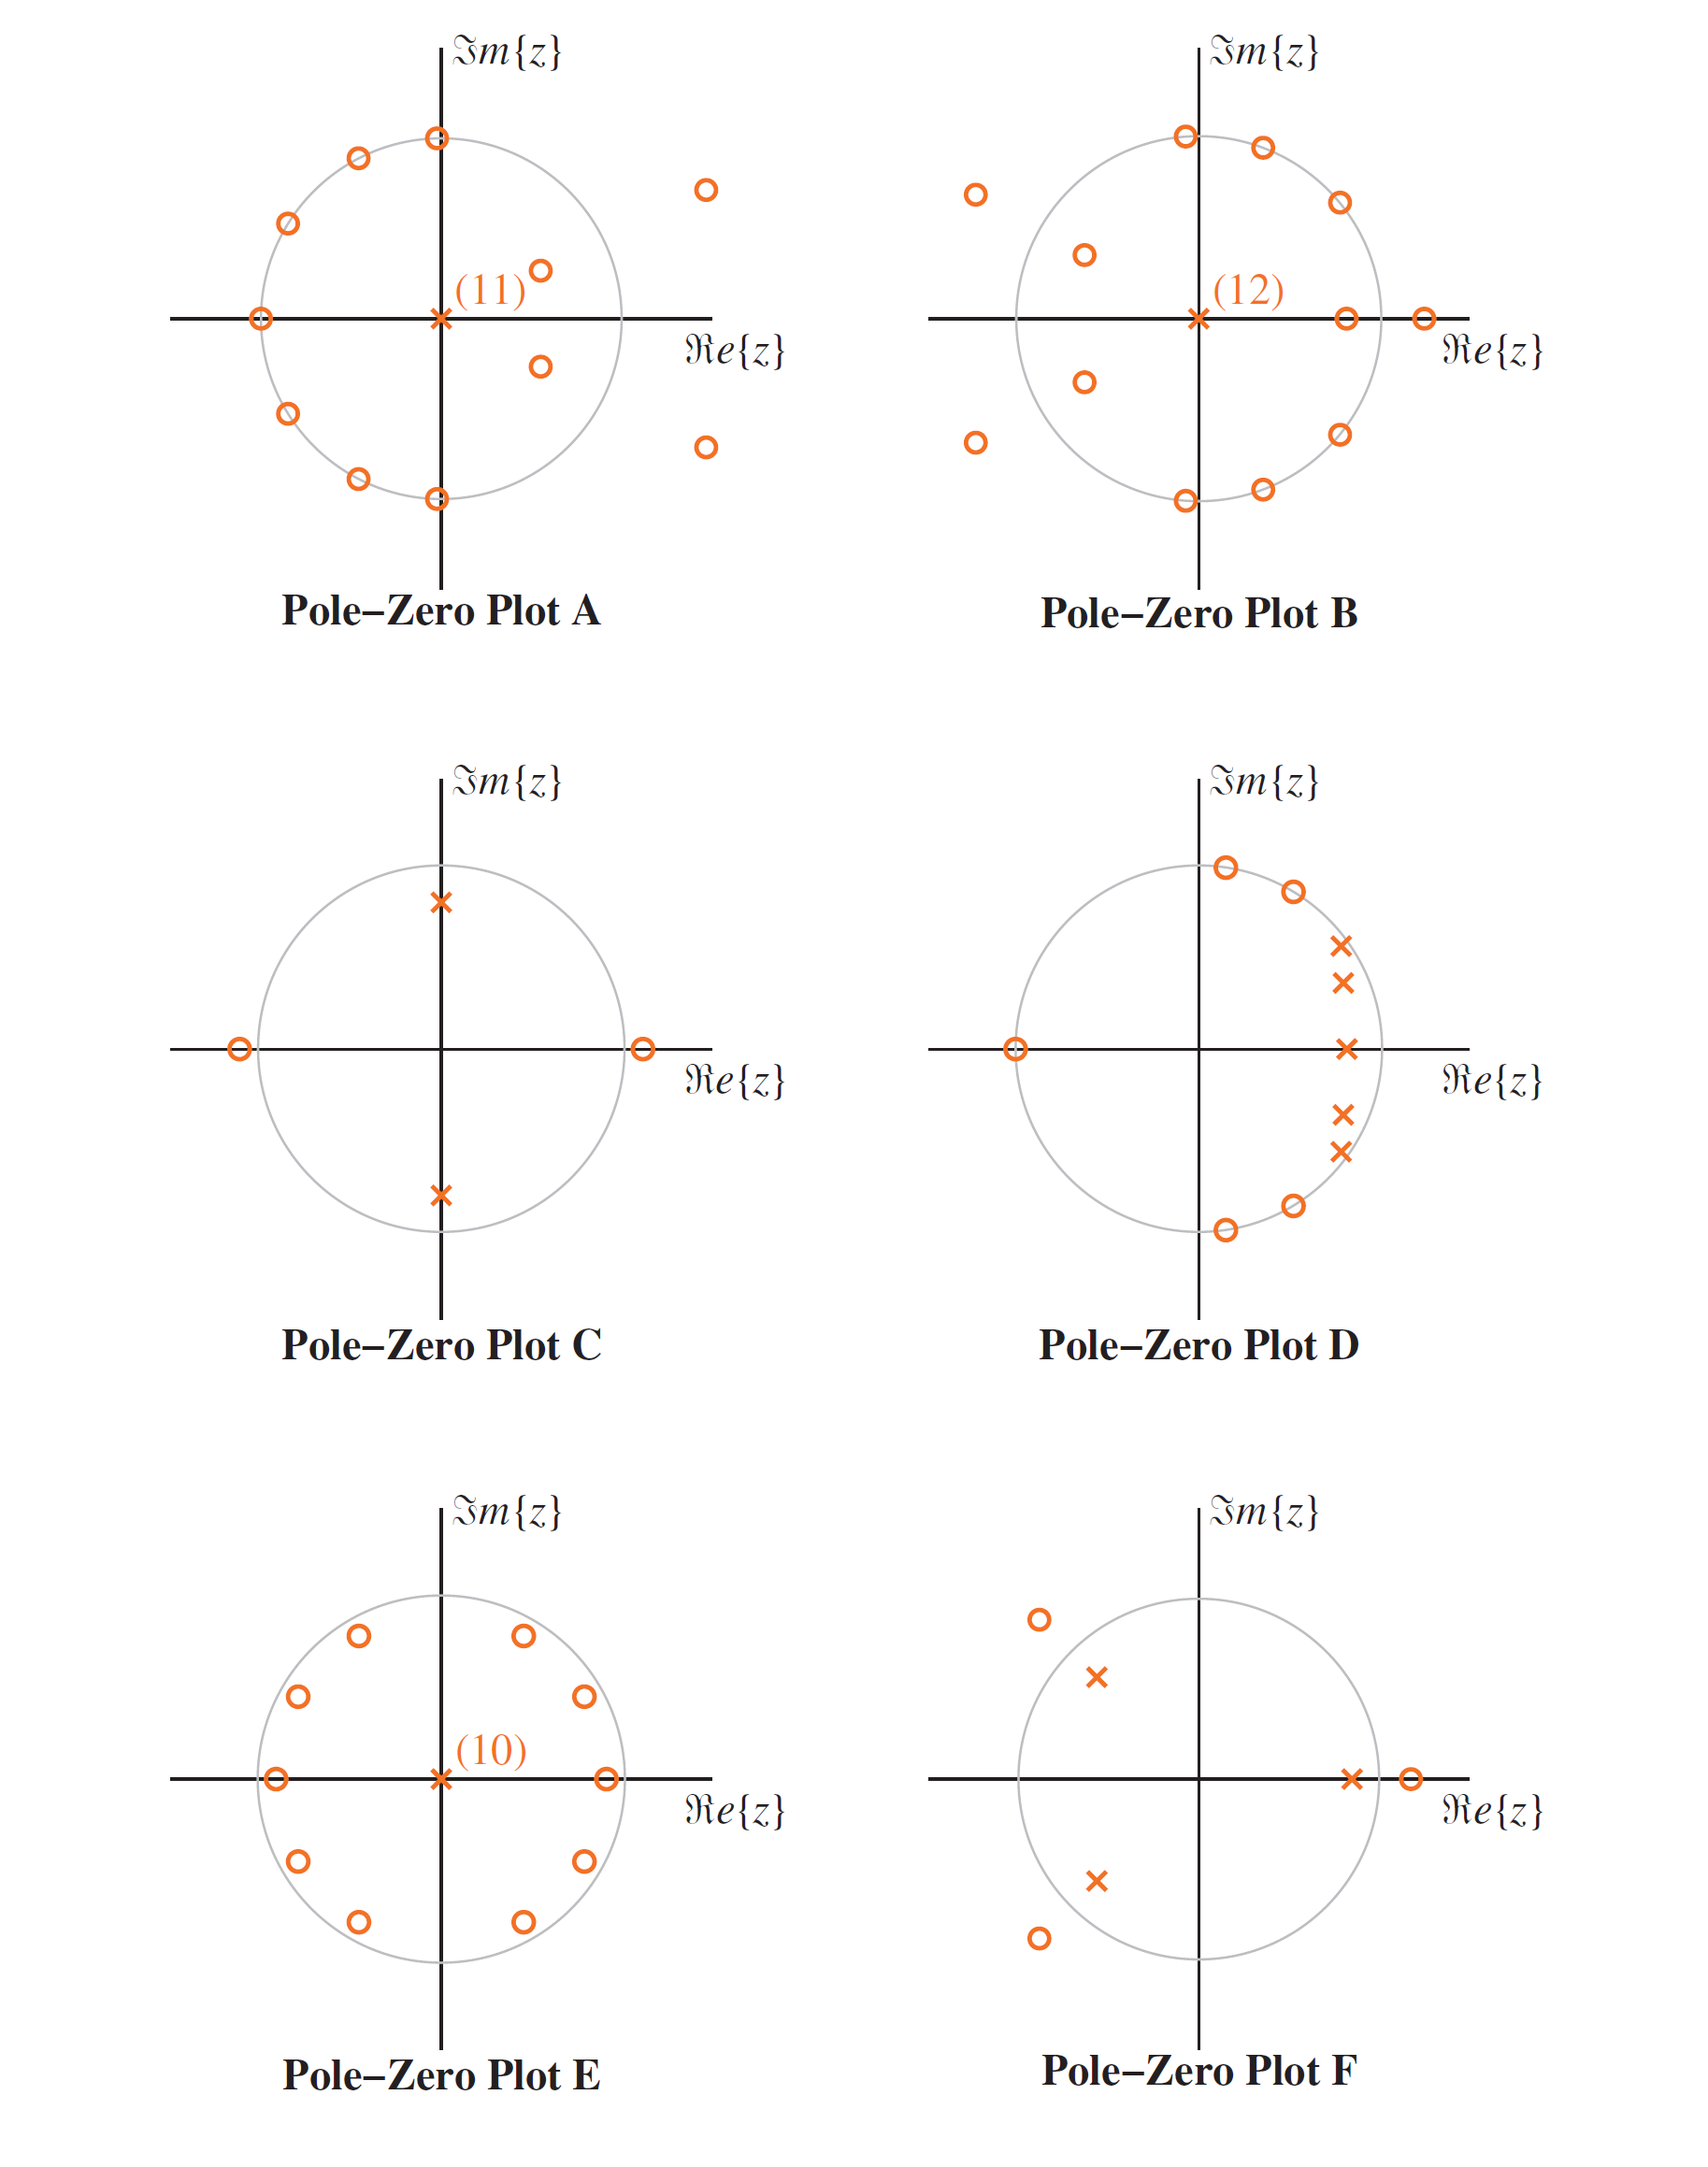
\includegraphics[scale=0.4]{figs/several_pole_zero_diagram.png}
	\caption{Pole-zero diagrams for problem 3. These diagrams describe six different \textbf{\underline{causal}} LTI systems; unit circle is shown for reference.}
	\label{fig:pole-zero-diagram}
\end{figure}


\newpage

\noindent {\bf Problem 4: Kramers-Kronig relations in discrete time (25 points)}

This problem will guide you through the proof of the Kramers-Kronig relations for \underline{discrete-time} signals, which establish that the real and imaginary parts of the DTFT of a \underline{real} and \underline{causal} signal $x[n] \Longleftrightarrow X(e^{j\omega}) = \mathrm{Re}\{X(e^{j\omega})\} + j\mathrm{Im}\{X(e^{j\omega})\}$ are related by 

\begin{align} \nonumber
\mathrm{Im}\{X(e^{j\omega})\} &= -\frac{1}{2\pi}\bigg[\Big(\frac{\sin\omega}{1-\cos\omega}\Big)\ast \mathrm{Re}\{X(e^{j\omega})\}\bigg] \\
&=-\frac{1}{2\pi}\int_{-\pi}^{\pi}\bigg(\frac{\sin\theta}{1-\cos\theta}\bigg)\mathrm{Re}\{X(e^{j(\omega-\theta)})\}d\theta
\end{align}

\noindent\textbf{Note:} This result looks a bit different from the one discussed in class, as in this problem you're working in discrete time. However, the same steps  can be followed to arrive at the result for continuous time. The only difference would be that in continuous time: $\mathcal{F}\{\mathrm{sign(t)}\} = -\frac{2j}{\Omega}, \Omega\neq 0$. Then, we would have
\begin{equation}
\mathrm{Im}\{X(j\Omega)\} = -\frac{1}{\pi\Omega}\ast \mathrm{Re}\{X(j\Omega)\} = -\mathcal{H}\{\mathrm{Re}\{X(j\Omega)\}\},
\end{equation}	
where this convolution is known as the Hilbert transform.


\begin{description}
	\item[(a)] \textbf{Even/odd decomposition}. Recall from lecture notes 1 that any signal $x[n] \leftrightarrow X(e^{j\omega})$ can be written as
	\begin{equation}
	x[n] = x_e[n] + x_o[n],
	\end{equation}
	where 
	\begin{align}
	x_e[n] = \frac{1}{2}(x[n] + x[-n]) \tag{even symmetric: $x_e[n] = x_e[-n]$} \\
	x_o[n] = \frac{1}{2}(x[n] - x[-n]) \tag{odd symmetric: $x_o[n] = -x_o[-n]$}
	\end{align}
	
	Assume that $x[n]$ is \underline{real} and write expressions for the DTFT of $x_e[n]$ and $x_o[n]$ as a function of $X(e^{j\omega})$.
	
	\textit{Hint:} Table 2.2 of the textbook lists useful properties of the DTFT.
	
	\item[(b)] Now assume that $x[n]$ is also \underline{causal} i.e., $x[n] = 0, n < 0$. Write an equation for $x_o[n]$ in terms of $x_e[n]$ only. Use this result to write an equation for $X_o(e^{j\omega}) = \mathcal{F}\{x_o[n]\}$ as a function of $X_e(e^{j\omega})=\mathcal{F}\{x_e[n]\}$ only.
	
	\textit{Hint:} You may use the following result:
	\begin{equation}
	\mathcal{F}\{\mathrm{sign[n]}\} = \begin{cases}
	-j\displaystyle\frac{\sin\omega}{1-\cos\omega}, &\omega\neq 0 \\
	0, &\omega = 0
	\end{cases}
	\end{equation} 
	
	\item[(c)] Combine your results of parts (a) and (b) to show that 
	
	\begin{equation}
	\mathrm{Im}\{X(e^{j\omega})\} = -\frac{1}{2\pi}\bigg[\Big(\frac{\sin\omega}{1-\cos\omega}\Big)\ast \mathrm{Re}\{X(e^{j\omega})\}\bigg]
	\end{equation}
\end{description} 

\newpage
\noindent \textbf{Attachment}\\
\rule{6.5 in}{0.5pt}

\begin{figure}[h!]
	\centering
	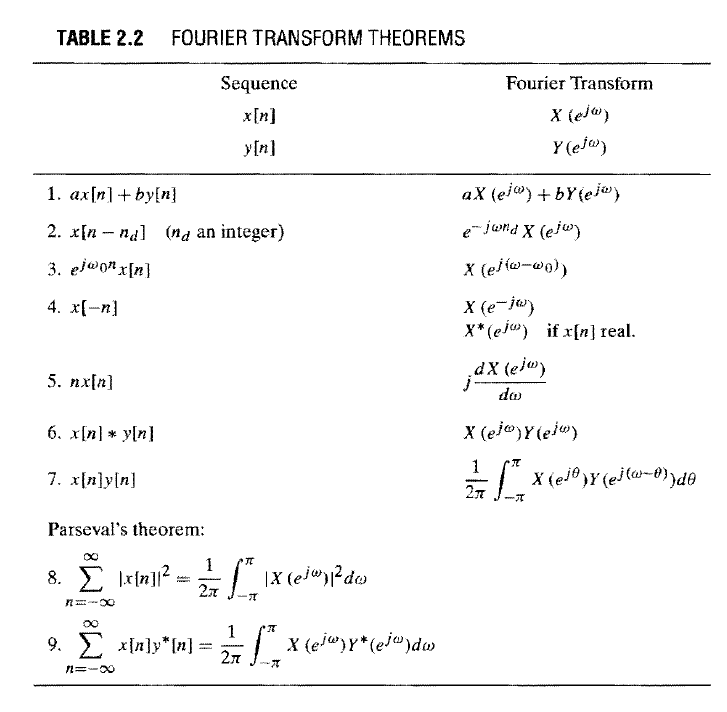
\includegraphics{figs/table22.png}
	\caption{Table 2.2 of the textbook.}
\end{figure}

\end{document}
